\documentclass[12pt]{article}

\usepackage{natbib}
\usepackage{amssymb}
\usepackage{amsmath}
\usepackage{bm}
\usepackage{dsfont}
\usepackage{multirow}
\usepackage[margin=1.25in]{geometry}
\usepackage[font=footnotesize]{caption}
\usepackage{dsfont}
\usepackage{amsmath}
\usepackage{graphicx}
\usepackage{bm}
\usepackage{enumerate}
\usepackage[shortlabels]{enumitem}
\newcommand{\m}[1]{\mathbf{\bm{#1}}}
\newcommand{\R}{I\hspace{-4.4pt}R}
\newcommand{\bc}[1]{\textcolor{blue}{\mathbf{#1}}}
\newcommand{\ind}{\mathds{1}}

%\setlength{\parindent}{0pt}

\begin{document}

\noindent AMS 268 -- Final Project

\noindent Mickey Warner
\bigskip
\bigskip

{\Large \noindent Bayesian linear regression and variable selection methods with large $n$}


\section{Introduction}

The content of this paper comes primarily from \cite{qian2017big}. Suppose we want to perform a regression on data $X,y$ using a linear model
\begin{align}
y = X \beta + \epsilon
\end{align}
where $y$ is $n\times 1$, $X$ is $n\times k$, $\beta$ is $k\times 1$, and $\epsilon\sim N(0, \sigma^2 I)$. We consider the case when $n$ is so large that we cannot hold all the data in memory or that certain necessary computations become infeasible. It may also be the case that the data is located on separate servers. The approach discussed here handles these issues.

\section{Methods}

We will consider $m$ subsets $(X_1,y_1),\ldots,(X_m,y_m)$ a partition of the full data $(X,y)$. Each subset is independent of all other subsets, and we also assume independence within each subset. Given a particular subset, computing the posterior distribution $\pi(\beta_i,\sigma_i^2|X_i, y_i)$ is much easier. Our goal is obtain the full posterior of $(\beta,\sigma^2)$ given all the data.

This is accomplished by placing a Normal-Inverse-Gamma (NIG) prior on $(\beta_i,\sigma_i^2)$. This distribution has density
\begin{align}
p(\beta, \sigma^2) \propto (\sigma^2)^{-(a+k/2+1)}e^{-\frac{1}{\sigma^2}\left[b+\frac{1}{2}(\beta-\mu)^\top \Lambda^{-1}(\beta-\mu)\right]}
\end{align}
written $NIG(\mu,\Lambda,a,b)$. If the non-informative prior $p(\beta,\sigma^2)\propto 1/\sigma^2$ is assumed, then the posterior for subset $i$ is $NIG(\mu_i,\Lambda_i,a_i,b_i)$ where
\begin{align}
\begin{split}
\mu_i &= (X_i^\top X_i)^{-1} X_i^\top y_i \\
\Lambda_i &= X_i^\top X_i \\
a_i &= \frac{n_i-k}{2} \\
b_i &= \frac{1}{2}y_i^\top y_i -\frac{1}{2}y_i^\top X_i (X_i^\top X_i)^{-1} X_i^\top y_i
\end{split}
\end{align}
with $n_i$ being the number of observations contained in subset $i$. The subsets should be chosen so the calculations in (3) are doable.

Under the prior just described, it is possible to compute the full posterior for $(\beta,\sigma^2)$ using Normal-Inverse-Gamma summation. Consider two $k$-dimensional distributions $NIG(\mu_1, \Lambda_1, a_1, b_1)$ and $NIG(\mu_2, \Lambda_2, a_2, b_2)$. If a distribution $NIG(\mu, \Lambda, a, b)$ satisfies
\begin{align}
\begin{split}
\mu &=(\Lambda_1+\Lambda_2)^{-1}(\Lambda_1\mu_1 + \Lambda_2\mu_2) \\
\Lambda &=\Lambda_1+\Lambda_2 \\
a &=a_1+a_2+\frac{k}{2} \\
b &=b_1+b_2+\frac{1}{2}(\mu_1-\mu_2)^\top(\Lambda_1^{-1}+\Lambda_2^{-1})^{-1}(\mu_1-\mu_2)
\end{split}
\end{align}
then it is said to be the sum of two NIG distributions
\begin{align}
NIG(\mu, \Lambda, a, b) = NIG(\mu_1, \Lambda_1, a_1, b_1) + NIG(\mu_2, \Lambda_2, a_2, b_2)
\end{align}
The NIG summation operator is commutative and associative, making it easy to sum up any number of NIG distributions, in any order. When new data arrives, the posterior distribution can easily be updated.

The algorithm to obtain the full posterior can be summarized as follows:
\begin{enumerate}
\item Partition the data into $m$ subsets $X_i,y_i$, $i=1,\ldots,m$
\item Obtain the subset posterior distributions under the non-informative prior using (3). This yields parameter estimates $\tilde{\mu_i}, \tilde{\Lambda_i}, \tilde{a_i}, \tilde{b_i}$.
\item Gather and sum the subset posteriors
\[ NIG(\tilde{\mu}, \tilde{\Lambda}, \tilde{a}, \tilde{b}) = \sum_{i=1}^m NIG(\tilde{\mu_i}, \tilde{\Lambda_i}, \tilde{a_i}, \tilde{b_i}) \]
\item Add any prior information
\[ NIG(\overline{\mu},\overline{\Lambda}, \overline{a}, \overline{b}) = NIG(\mu,\Lambda,a,b)+NIG(\tilde{\mu}, \tilde{\Lambda}, \tilde{a}, \tilde{b}) \]
to obtain the full posterior distribution.
\end{enumerate}

\subsection{LASSO, SSVS, MC$^3$}

The above algorithm acts as a starting point for other models. First run the algorithm, then use the posterior for $(\beta,\sigma^2)$ to update other parameters included in the desired model. This is likely to be done iteratively or in an MCMC fashion.

In LASSO, there is a parameter that adjusts the precision $\Lambda$ to account for an $L_1$ penalty in $\beta$. For stochastic search variable selection (SSVS) and MCMC model composition (MC$^3$), there are parameters $\gamma_j\in\{0,1\}$, for $j=1,\ldots,k$ which denote whether $\beta_j$ ought to be included in the model (1). The difference between these two models is that in MC$^3$ when a $\gamma_j=0$ (i.e., covariate $j$ not included), then an adjustment to (1) is made so the corresponding $\beta_j$'s are zero and the respective columns in $X$ are removed. The posterior mean of $\gamma_j$ informs us of the proportion of times covariate $j$ was included in the model. The effect of this is made evident in the subsequent simulation study.

The use of the full posterior of $(\beta,\sigma^2)$ suggests that it is possible to fit any model, provided the data are not required beyond obtaining $(\beta,\sigma^2)$ via the above algorithm. Some of these models are presented in \cite{qian2017big}. Refer to that paper for more details on LASSO, SSVS, and MC$^3$.

\section{Simulation study}

We simulate $n=1,000,000$ samples from the model
\begin{align}
y_i \sim N(x_i^\top, \beta, \sigma^2),~~~~~i=1,\ldots,n
\end{align}
where $x_i$ follows a mean-zero $k$-variate normal distribution with all variances $1$ and all correlations $\rho$, with $k=40$. We set $\beta=(1, 0.9, \ldots, 0.1, 0, \ldots, 0)^\top$. The data are split into $m=100$ subsets. In our case, the $n$ is relatively small so the analysis can be performed on a single machine, but the method extends easily to very large $n$.

Simulations are made with $\rho=0, 0.99$ and $\sigma=1, 10$, making a total of four combinations.

\section{Results}

Coefficient esimates and several model comparison features are given on the next two pages. MC$^3$ performs just as well or better than the other three models in every case. When $\rho\neq 0.99$ and $\sigma\neq 10$, estimates for $\beta$ are nearly identical. Every model is trouble estimate $\beta$ when $\rho=0.99$, particularly those $\beta_j$'s close, not equal, to zero. And only when $\rho=0.99$ and $\sigma=10$ does MC$^3$ struggle selecting the correct variables, while $SSVS$ has difficulty even in not crazy cases. But this could possibly be improved by using a better prior for $\gamma_j$.

\begin{figure}[H]
\begin{center}
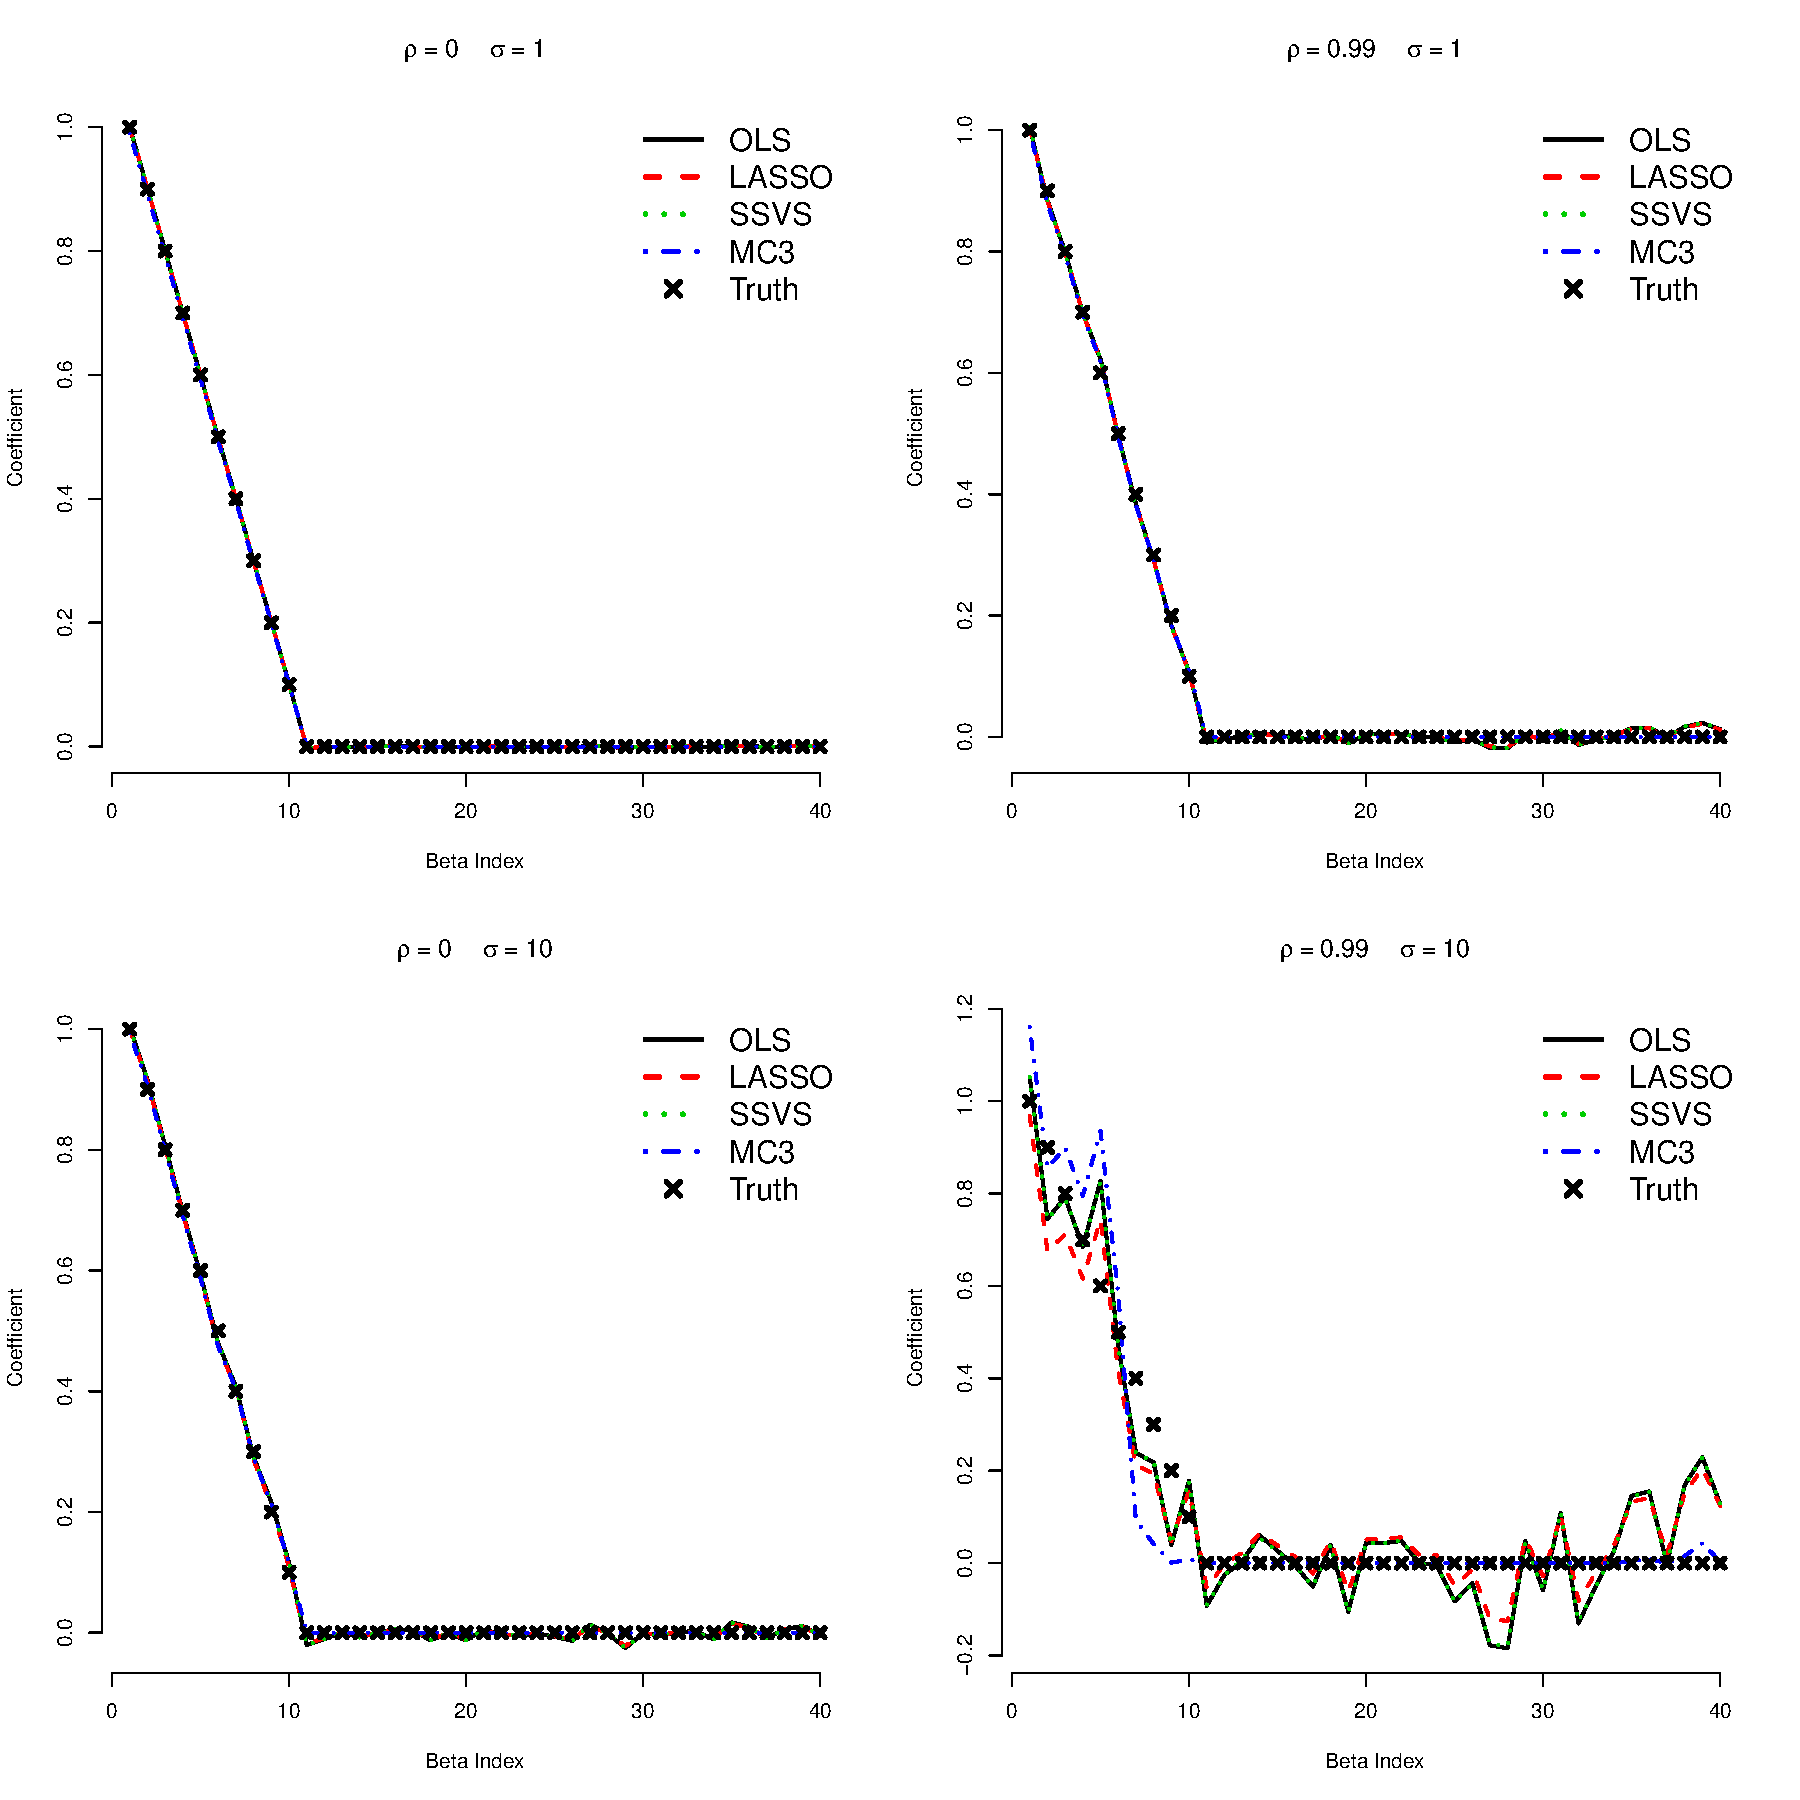
\includegraphics[scale=0.5]{../figs/four_estimates.pdf}
\end{center}
\caption{Posterior means for $\beta$ for each algorithm, under each setting.}
\end{figure}

\begin{table}[H]
\centering
\begin{tabular}{lrrrr}
  \hline\hline
 & OLS & LASSO & SSVS & MC3 \\ 
  \hline
$\rho=0$, $\sigma=1$     & -13.08 & -13.13 & -13.08 & -11.57 \\ 
$\rho=0.99$, $\sigma=1$  & -8.49 & -8.58 & -8.47 & -9.57 \\ 
$\rho=0$, $\sigma=10$    & -8.48 & -8.40 & -8.47 & -9.65 \\ 
$\rho=0.99$, $\sigma=10$ & -3.88 & -3.78 & -3.89 & -4.39 \\ 
   \hline\hline
\end{tabular}
\caption{Log MSE for $\beta$}
\end{table}

\begin{table}[H]
\centering
\begin{tabular}{llrrrr}
  \hline\hline
& & OLS & LASSO & SSVS & MC3 \\ 
  \hline
\multirow{4}{*}{Non-zero} & $\rho=0$, $\sigma=1$     & 0.004 & 0.004 & 0.004 & 0.004 \\ 
                          & $\rho=0.99$, $\sigma=1$  & 0.039 & 0.039 & 0.039 & 0.042 \\ 
                          & $\rho=0$, $\sigma=10$    & 0.039 & 0.064 & 0.039 & 0.039 \\ 
                          & $\rho=0.99$, $\sigma=10$ & 0.386 & 0.658 & 0.386 & 0.326 \\ \hline
\multirow{4}{*}{Zero} & $\rho=0$, $\sigma=1$     & 0.004 & 0.004 & 0.004 & 0.000 \\ 
                      & $\rho=0.99$, $\sigma=1$  & 0.039 & 0.037 & 0.038 & 0.000 \\ 
                      & $\rho=0$, $\sigma=10$    & 0.039 & 0.038 & 0.039 & 0.000 \\ 
                      & $\rho=0.99$, $\sigma=10$ & 0.387 & 0.368 & 0.385 & 0.030 \\ 
   \hline\hline
\end{tabular}
\caption{Mean 95\% posterior interval length of $\beta$, separated by those $\beta$'s which are truly non-zero and zero.}
\end{table}

\begin{table}[ht]
\centering
\begin{tabular}{lrrrr}
  \hline\hline
 & OLS & LASSO & SSVS & MC3 \\ 
  \hline
$\rho=0$, $\sigma=1$     & 0.95 & 0.96 & 0.95 & 0.96 \\ 
$\rho=0.99$, $\sigma=1$  & 0.96 & 0.95 & 0.95 & 0.98 \\ 
$\rho=0$, $\sigma=10$    & 0.95 & 0.96 & 0.96 & 0.96 \\ 
$\rho=0.99$, $\sigma=10$ & 0.96 & 0.95 & 0.95 & 0.95 \\ 
   \hline\hline
\end{tabular}
\caption{Coverage of prediction intervals on a new data set.}
\end{table}

\begin{table}[ht]
\centering
\begin{tabular}{llrrrrrrrrrrr}
  \hline\hline
 & & \multicolumn{10}{c}{$j$} \\
 & & 1 & 2 & 3 & 4 & 5 & 6 & 7 & 8 & 9 & 10 \\ 
  \hline
\multirow{2}{*}{$\rho=0$, $\sigma=1$} & SSVS & 1.00 & 1.00 & 1.00 & 1.00 & 1.00 & 0.96 & 0.24 & 0.01 & 0.00 & 0.00 \\ 
 & MC3  & 1.00 & 1.00 & 1.00 & 1.00 & 1.00 & 1.00 & 1.00 & 1.00 & 1.00 & 1.00 \\  \hline
\multirow{2}{*}{$\rho=0.99$, $\sigma=1$} & SSVS & 1.00 & 1.00 & 1.00 & 1.00 & 1.00 & 0.96 & 0.14 & 0.01 & 0.00 & 0.00 \\ 
 & MC3  & 1.00 & 1.00 & 1.00 & 1.00 & 1.00 & 1.00 & 1.00 & 1.00 & 1.00 & 1.00 \\  \hline
\multirow{2}{*}{$\rho=0$, $\sigma=10$} & SSVS & 1.00 & 1.00 & 1.00 & 1.00 & 1.00 & 0.91 & 0.31 & 0.01 & 0.00 & 0.00 \\ 
 & MC3  & 1.00 & 1.00 & 1.00 & 1.00 & 1.00 & 1.00 & 1.00 & 1.00 & 1.00 & 1.00 \\  \hline 
\multirow{2}{*}{$\rho=0.99$, $\sigma=10$} & SSVS & 1.00 & 1.00 & 1.00 & 0.99 & 1.00 & 0.66 & 0.04 & 0.03 & 0.00 & 0.01 \\ 
 & MC3  & 1.00 & 1.00 & 1.00 & 1.00 & 1.00 & 1.00 & 0.28 & 0.13 & 0.01 & 0.03 \\ 
   \hline\hline
\end{tabular}
\caption{Posterior mean $E(\gamma_j|\cdot)$.}
\end{table}






\bibliography{refs}
\bibliographystyle{asa}

\end{document}
